\subsection{Entity Relationship Class Diagram }
\label{sub:db}


The underlying database structure of the developed application is mostly influenced by the \gls{SKB} and the representation of \texttt{Assumptions} as classes. \autoref{fig:er} shows an overview over most of the involved database models used in this application. Additional classes like \texttt{Users}, \texttt{Abilities}, etc. are intentionally left out to reduce complexity. 

\begin{sidewaysfigure*}
	\centering
	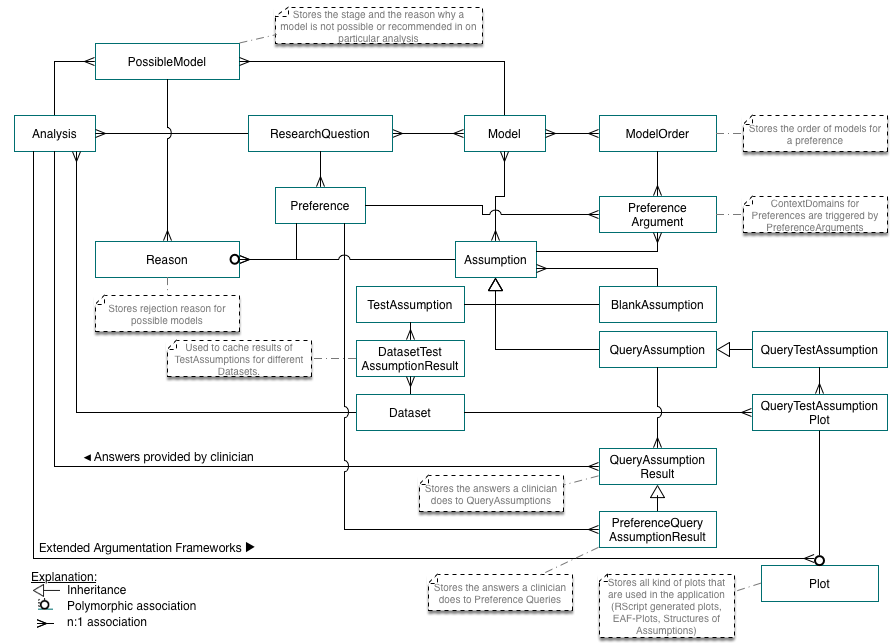
\includegraphics[width=0.9\textwidth]{figures/er_complete}
	\caption{Entity-Relationship Diagram of the major classes used in the application. }
	\label{fig:er}
\end{sidewaysfigure*}


The most important class is \texttt{Analysis} which is associated with \texttt{Dataset} and \texttt{Research-} \texttt{Question}. It has many answered or open \texttt{QueryAssumptionResults}\footnote{This class stores the answers of a clinician to one particular \texttt{QueryAssumption}} and a list of \texttt{PossibleModels} (including impossible models and their \texttt{Reason} why they got rejected). \texttt{ResearchQuestions} have and belong to many \texttt{Models}. Each of these has multiple \texttt{Assumptions} that need to hold for its \texttt{Model}. These \texttt{Assumptions} have different specialisations: 

\bigskip

\begin{itemize}

	\item \texttt{TestAssumption}: An assumption that requires an \texttt{R}-script to be executed and to return \texttt{true} or \texttt{false}. These assumptions will be checked automatically by the system and rely only on the data set used in an analysis.
	\item \texttt{QueryAssumption}: A clinician has to provide a \textit{yes} or \textit{no} answer to a question during the process of the analysis. Only if he answers positively, this assumption holds.
	\item \texttt{QueryTestAssumption}: An \texttt{R}-script generates a plot based on the data set, which is then presented to the user who has to confirm, that the plot shows some required features.
	\item \texttt{BlankAssumption}: An assumption that represents a grouping ability for other assumptions. All assigned assumptions (regardless of their type) must hold. 
\end{itemize}
\bigskip


\texttt{Preferences} have different \texttt{PreferenceArguments} that represent a specific \gls{CD} which are assigned to a particular \texttt{ModelOrder}. This allows the representation of \glspl{CD}, their order and the expressed preferences as described in \autoref{sub:SKB} in a generic way without limiting the triggers for a \gls{CD} to any particular \texttt{Assumption} type. 

The class \texttt{DatasetTestAssumptionResult} stores for each \texttt{TestAssumption} and each \texttt{Dataset} a pre-calculated result to enhance the speed of the evaluation during new \texttt{Analses}. \texttt{PreferenceQueryAssumptionResults} and \texttt{QueryAssumptionResults} store the answers of clinicians to \texttt{(Test)QueryAssumptions} for one particular \texttt{Analysis}.
